\chapter{LFT: Lattice with Fermions}\label{ch:ferm}

We will now introduce Fermions on the lattice. Parts of this presentation 
follows Chapters 5 and 10 of~\cite{gattringer_quantum_2010}. 
We will start in the continuum
and introduce a naive discretization. Then we will go into detail, point
out a problem with the naive discretization, and fix it. We will omit
space-time dependence sometimes for the sake of brevity, but it should
be clear which objects have space-time dependence anyway. Primarily
we are interested in studying QCD, so $N_c=3$. This chapter uses Dirac
algebra extensively, but the algebra is different when the metric
is Euclidean. For details see \apref{ap:spec_math}.

In the continuum theory, the free fermion action is 
\begin{equation}
  S_F=\int\dd[4]{x}\bar{\psi}(\slashed{\partial}+m)\psi.
\end{equation}
Using the rules~\eqref{eq:dertodiff} and \eqref{eq:inttosum}, one naively
discretizes this action on the lattice as
\begin{equation}\label{eq:naivefermact}
  S_F=a^4\sum_x\bar{\psi}(x)\left(\sum_{\mu=1}^4\gamma_\mu
       \frac{\psi(x+a\hat{\mu})-\psi(x-a\hat{\mu})}{2a}
       +m\psi(x)\right).
\end{equation}
The fermionic partition function is
\begin{equation}
  Z_F=\int\DD{\psi}\DD{\bar{\psi}}e^{-S_F},
\end{equation}
with integration measure
\begin{equation}
  \int\DD{\psi}\DD{\bar{\psi}}
   =\prod_{x,f,\alpha,c}\dd{\bar{\psi}^f_{\alpha c}(x)}
                        \dd{\psi^f_{\alpha c}(x)},
\end{equation}
where $f$ runs over flavors, $\alpha$ runs over Dirac indices, and $c$
runs over colors.\footnote{We will try in this book to follow the convention of
Ref.~\cite{gattringer_quantum_2010} and indicate Dirac indices with Greek
letters and color indices with Latin letters.}

In addition, we want the fermionic action to be gauge invariant. The
gauge transformation for fermion fields
\begin{equation}
  \psi(x)\to U(x)\psi(x),~~~~~\bar{\psi}(x)\to\bar{\psi}(x)U(x)^\dagger
\end{equation}
with $U\in\SU(3)$ reminds us of the gauge transformation for scalar 
fields given in Chapter~\ref{ch:preliminaries}. Working in the continuum 
we introduce, just as before, a gauge field $A_\mu(x)$ so that the 
fermionic action becomes
\begin{equation}
  S_F=\int\dd[4]{x}\bar{\psi}\big(\gamma_\mu(\partial_\mu+A_\mu)+m\big)\psi.
\end{equation}
The gauge-transformed fermionic action is
\begin{equation}
  S'_F=\int\dd[4]{x}\bar{\psi}\,U^\dagger
        \big(\gamma_\mu(\partial_\mu+A'_\mu)+m\big)U\psi,
\end{equation}
so that the requirement of gauge invariance leads us to conclude
\begin{equation}
  (\partial_\mu+A_\mu)\psi=U^\dagger(\partial_\mu+A'_\mu)U\psi.
\end{equation}
Solving for $A'_\mu$ we find
\begin{equation}
  A'_\mu=(\partial_\mu U)U^\dagger-UA_\mu U^\dagger,
\end{equation}
just as with the pure gauge case. 

On the lattice, link variables transform as
\begin{equation}
  U_\mu(x)\to U'_\mu(x)=U(x)U_\mu(x)U^\dagger(x+a\hat{\mu}),
\end{equation}
which ensures that closed loops of link variables are gauge invariant.
In addition the discretized fermionic action becomes gauge invariant
when it is written as
\begin{equation}\label{eq:naivefermactgauge}
  S_F=a^4\sum_x\bar{\psi}(x)\left(\sum_{\mu=1}^4\gamma_\mu
       \frac{U_\mu(x)\psi(x+a\hat{\mu})-U_{-\mu}(x)\psi(x-a\hat{\mu})}{2a}
       +m\psi(x)\right),
\end{equation}
where
\begin{equation}
  U_{-\mu}(x)=U_\mu(x-a\hat{\mu})^\dagger
\end{equation}
transforms as
\begin{equation}
  U_{-\mu}(x)\to U'_{-\mu}(x)=U(x)U_{-\mu}(x)U^\dagger(x-a\hat{\mu}).
\end{equation}
Since \equatref{eq:naivefermactgauge} is the gauge-invariant action,
this will be what we investigate for fermion doubling.

In this chapter, it will be convenient to separate out fermionic and gluonic
parts of the path integral. To this end, we factorize expectation values as
\begin{equation}\label{eq:evfact}
\ev{...}=\ev{\ev{...}_F}_G.
\end{equation} 
For an observable $X$, the fermionic expectation value is defined as
\begin{equation}\label{eq:evferm}
\ev{X}_F\equiv\frac{1}{Z_F(U)}\int\DD\psi\DD\bar\psi
e^{-S_F\left(\bar\psi,\psi,U\right)} X\left(\bar\psi,\psi,U\right),~~~~~
Z_F(U)=\int\DD\psi\DD\bar\psi e^{-S_F\left(\bar\psi,\psi,U\right)}.
\end{equation}
This expectation value thus integrates out the fermionic degrees of freedom,
leaving only a dependence on the gauge field.
With this definition, the gluonic expectation value must be
\begin{equation}
\ev{X}_G\equiv\frac{1}{Z}\int\DD U e^{-S_G} Z_F(U) X(U)
\end{equation}
so that
\begin{equation}
\ev{X}=\frac{1}{Z}\int\DD U\DD\psi\DD\bar\psi
e^{-S_G(U)-S_F\left(\bar\psi,\psi,U\right)} X\left(\bar\psi,\psi,U\right)
\end{equation}
as expected.

\section{Grassmann numbers}\label{sec:grassmann}\index{algebra!Grassmann}
\index{Grassmann!algebra}
Fermions are objects that by definition anticommute with each other. 
With this in mind, we introduce Grassmann numbers.
We consider a set of numbers $\eta_i$, $1\leq i\leq N$ obeying
\begin{equation}
  \eta_i\eta_j=-\eta_j\eta_i
\end{equation}
for all $i$ and $j$. These are called {\it Grassmann
numbers}\index{Grassmann!number}.
It follows that
\begin{equation}\label{eq:gnilpotent}
  \eta_i^2=0.
\end{equation}
If a power series of a function $f$ of the Grassmann numbers exists, then
\equatref{eq:gnilpotent} guarantees that the series terminates almost
immediately. In general we would write
\begin{equation}\label{eq:grasspoly}
  f(\eta)=a+\sum_ia_i\eta_i+\sum_{i<j}a_{ij}\eta_i\eta_j
           +...+a_{1...N}\eta_1...\eta_N
\end{equation}
with $a,\,a_i,\,a_{ij},...,\,a_{1...N}\in\mathbb{C}$.
We refer to \equatref{eq:grasspoly} as a {\it Grassmann polynomial}.
Grassmann\index{Grassmann!polynomial} 
polynomials are closed under addition and multiplication,
and are thus said to form a {\it Grassmann algebra}. The $\eta_i$
are the {\it generators} of the Grassmann algebra.

To learn how differentiation ought to work, we use the simple example
$N=2$. Then
\begin{equation}
  f(\eta)=a+a_1\eta_1+a_{12}\eta_1\eta_2.
\end{equation}
A definition of the derivative that follows our intuition is
\begin{equation}
  \pdv{f}{\eta_1}=a_1+a_{12}\eta_2.
\end{equation}
However, the defining characteristic of Grassmann numbers is that they
anticommute. Therefore we could also have expanded $f$ as
\begin{equation}
  f(\eta)=a+a_1\eta_1-a_{12}\eta_2\eta_1.
\end{equation}
In order for the derivative $f$ to make sense we must therefore require
\begin{equation}
  \pdv{\eta_1}\eta_2=
  -\eta_2\pdv{\eta_1}.
\end{equation}
Similarly if we take another derivative, this time with respect to $\eta_2$,
we find that partial derivatives with respect to different Grassmann variables
must also anticommute to maintain consistency. Altogether, the differentiation
rules for Grassmann variables become
\begin{equation}\begin{aligned}
  \pdv{\eta_i}1&=0;\\
  \pdv{\eta_i}\eta_i&=1;\\
  \pdv{\eta_i}\eta_j&=
  -\eta_j\pdv{\eta_i};\\
  \frac{\partial^2}{\partial\eta_i\partial\eta_j}&=
  -\frac{\partial^2}{\partial\eta_j\partial\eta_i}.
\end{aligned}\end{equation}

Next we move on to integration. We will construct integrals that work like
integrals over subsets $\Omega\in\mathbb{R}^N$ for which 
the integrand vanishes at the boundary $\partial\Omega$. 
Thus we demand that the Grassmann integral is a complex number,
\begin{equation}
  \int\dd[N]{\eta}f\in\mathbb{C};
\end{equation}
that with $\lambda_1,\lambda_2\in\mathbb{C}$ it is linear,
\begin{equation}\label{eq:grasslin}
  \int\dd[N]{\eta}\left(\lambda_1f_1+\lambda_2f_2\right)
       =\lambda_1\int\dd[N]{\eta}f_1
         +\lambda_2\int\dd[N]{\eta}f_2;
\end{equation}
and that its integrand vanishes at the boundary,
\begin{equation}\label{eq:grassBC}
  \int\dd[N]{\eta}\pdv{\eta_i}f=0.
\end{equation}
If some function $f$ of $N-1$ Grassmann numbers can be written as the 
derivative of another function $g$ of $N$ Grassmann numbers, it follows
from \equatref{eq:grassBC} that the integrand vanishes.
An integral of a Grassmann polynomial of $N$ variables is therefore
proportional to the coefficient $a_{1...N}$, since
$\eta_1...\eta_N$ cannot be written as a derivative of $N$ variables.
In particular if we demand a normalization
\begin{equation}\label{eq:grassnorm}
  \int\dd[N]{\eta}\eta_1...\eta_N=1,
\end{equation}
we obtain the rule
\begin{equation}
  \int\dd[N]{\eta}f=a_{1...N}.
\end{equation}
Finally to make Grassmann integration more analogous to the integration that
we're used to, we define
\begin{equation}
  \dd[N]{\eta}\equiv\dd{\eta_N}...\dd{\eta_1}.
\end{equation}
Altogether then, the rules of Grassmann integration can be summarized by
\equatref{eq:grasslin} along with
\begin{equation}\label{eq:grassintrules}\begin{aligned}
       \int\dd{\eta_i}1&=0;\\
  \int\dd{\eta_i}\eta_i&=1;\\
  \dd{\eta_i}\dd{\eta_j}&=-\dd{\eta_j}\dd{\eta_i}.
\end{aligned}\end{equation}
Using these properties we can define integration over subsets of Grassmann
variables. Interestingly, the measures obey the same algebraic properties as
the derivatives.

Next let us discuss how Grassmann integrals behave under linear
transformations. In general we can write such a change of variables as
\begin{equation}\label{eq:grassxform}
  \eta'_i=M_{ij}\eta_j,
\end{equation}
where $M$ is a complex $N\times N$ matrix. More succinctly, one writes 
$\eta'=M\,\eta$. Applying this change of variables to the normalization
\equatref{eq:grassnorm} we obtain
\begin{equation}\begin{aligned}
  \int\dd[N]{\eta}\eta_1...\eta_N
     &=1\\
     &=\int\dd[N]{\eta'}\eta'_1...\eta'_N\\
     &=\int\dd[N]{\eta'}M_{1\,i_1}...M_{N\,i_N}\,\eta_{i_1}...\eta_{i_N}\\
     &=\int\dd[N]{\eta'}M_{1\,i_1}...M_{N\,i_N}\,\epsilon_{i_1...i_N}
               \eta_1...\eta_N\\
     &=\int\dd[N]{\eta'}\det M\,\eta_1...\eta_N.
\end{aligned}\end{equation}
It follows that under the transformation~\eqref{eq:grassxform}, the measure
transforms according to the rule
\begin{equation}
  \dd[N]{\eta}=\det M\dd[N]{\eta'},
\end{equation}
which is in some sense the ``opposite" of the usual transformation rule, where
the $\det M$ would have been on the LHS.

The stuff between the parentheses in the naive action~\eqref{eq:naivefermact}
can be viewed as an operator. Keeping this in mind, we're going to show
that the fermionic partition function can be viewed as a determinant.
The setup is as follows: We have a Grassmann algebra with $2N$ generators
$\bar{\eta}_i$ and $\eta_i$ that all anticommute with each other and
an $N\times N$ linear transformation $M$.
\begin{theorem}{Matthews-Salam formula}{}
\index{Matthews-Salam formula}
$$
  \int\prod_{i=1}^N\dd{\eta_i}\dd{\bar{\eta}_i}e^{\bar{\eta}M\eta}=\det M.
$$
\begin{proof} Let $\eta'=M\eta$. Then from \equatref{eq:grassxform}
  we have
  \begin{equation*}\begin{aligned}
  \int \prod_{i=1}^N\dd{\eta_i}\dd{\bar{\eta}_i}e^{\bar{\eta}M\eta}
    &=\det M\int \prod_{i=1}^N\dd{\eta'_i}\dd{\bar{\eta}_i}
       \exp\left(\sum_{j=1}^N\bar{\eta}_j\eta'_j\right)\\
    &=\det M\int \prod_{i=1}^N\dd{\eta'_i}\dd{\bar{\eta}_i}
       \exp\left(\bar{\eta}_i\eta'_i\right)\\
    &=\det M\int \prod_{i=1}^N\dd{\eta'_i}\dd{\bar{\eta}_i}
        (1+\bar{\eta}_i\eta'_i)\\
    &=\det M.
  \end{aligned}\end{equation*}
  The second line follows since pairs $\bar{\eta}_i\eta_i$ commute with
  each other, the third line is a power series expansion of the second
  line, and the last line follows from \equatref{eq:grassintrules}.
\end{proof}
\end{theorem}

Let us take a moment to see how the Matthews-Salam formula is employed
in lattice field theory. In our case, our Grassman variables are
fermion fields. The integration measure is a product over all
space-time sites, so that the index $i$ labels the site.
The matrix that occurs for us is the 
{\it Dirac operator}\index{Dirac!operator}
or {\it Dirac matrix}\index{Dirac!matrix} $D(x,y)$, appearing
in the action like
\begin{equation}\label{eq:diracPositionBasis}
\bar{\psi}(x)\left(\slashed{D}+m\right)\psi(y)
\equiv\bar{\psi}(x)D(x,y)\psi(y).
\end{equation}
Remember that $\slashed{D}$ contains a covariant derivative, which
is responsible for parallel transport between $x$ and its neighbors,
which is why we write $D(x,y)$. When we write $D(x,y)$, we are
now thinking about $\slashed{D}+m$ as a matrix in the basis
of spacetime points. The form of $D(x,y)$ will depend on how we
discretize\footnote{For example the Wilson action, which we will discuss
in \secref{sec:LFTdoubling}, has Kronecker $\delta$-functions that
enforce each site only interacts with its immediate neighbors.
In that sense the Wilson Dirac operator is ``tridiagonal".
The HISQ action on the other hand, which we will discuss in 
\secref{sec:HISQ}, includes interactions between sites and
their next-to-nearest neighbors. This is analogous to having a 
band diagonal matrix.}. Hence Matthews-Salam will let us trade
away the fermion fields for the determinant of the Dirac operator.
Due to the incredible size of $D(x,y)$, computing its determinant
is prohibitively computationally expensive. We will discuss the most
commonly used trick to avoid this in \secref{sec:pseudofermions}.

If we replace $M$ with the Dirac operator, we see that the fermionic
partition function is just the determinant of the Dirac operator.
By the way, the ordering of the differentials in the measure should
be $\dd{\eta}\dd{\bar{\eta}}$. This is because the $\bar{\eta}$ variables
in the integrand will always come on the left. By placing the
$\dd{\bar{\eta}}$ differentials on the right, it will always hit the
$\bar{\eta}$ variables first.

A generalization of this gives us the generating functional
for fermions. Here we consider $4N$ Grassmann numbers $\bar{\eta}_i$,
$\eta_i$, $\bar{\theta}_i$, and $\theta_i$. The $\bar{\theta}_i$
and the $\theta_i$ are the source terms. We define
\begin{equation}\label{eq:deffermgf}
  W[\theta,\bar{\theta}]\equiv\int \prod_{i=1}^N\dd{\bar{\eta}_i}\dd{\eta_i}
   e^{\bar{\eta}M\eta+\bar{\theta}\eta+\bar{\eta}\theta}
\end{equation}
\begin{theorem}{}{fermgf}
$$
   W[\theta,\bar{\theta}]=e^{-\bar{\theta}M^{-1}\theta}\det M.
$$
\begin{proof} Using the definition of the generating functional and
completing the square, we have 
$$
  \int \prod_{i=1}^N\dd{\bar{\eta}_i}\dd{\eta_i}
   e^{\bar{\eta}M\eta+\bar{\theta}\eta+\bar{\eta}\theta}
   =\int \prod_{i=1}^N\dd{\bar{\eta}_i}\dd{\eta_i}
   e^{(\bar{\eta}+\bar{\theta}M^{-1})\,M\,
             (\eta+M^{-1}\theta)-\bar{\theta}M^{-1}\theta}.
$$
Now we define new variables $\bar{\eta}'=\bar{\eta}+\bar{\theta}M^{-1}$
and $\eta'=\eta+M^{-1}\theta$. From \equatref{eq:grassintrules} it follows
that
$$
  \int \prod_{i=1}^N\dd{\bar{\eta}_i}\dd{\eta_i}=
  \int \prod_{i=1}^N\dd{\bar{\eta}'_i}\dd{\eta'_i}.
$$
Therefore by the Matthews-Salam formula,
\begin{equation*}\begin{aligned}
   \int \prod_{i=1}^N\dd{\bar{\eta}_i}\dd{\eta_i}
   e^{(\bar{\eta}+\bar{\theta}M^{-1})\,M\,
             (\eta+M^{-1}\theta)-\bar{\theta}M^{-1}\theta}
   &=\int \prod_{i=1}^N\dd{\bar{\eta}'_i}\dd{\eta'_i}
    e^{\bar{\eta}'M\eta'-\bar{\theta}M^{-1}\theta}\\
   &=e^{-\bar{\theta}M^{-1}\theta}\det M.
\end{aligned}\end{equation*}
\end{proof}
\end{theorem}
With the knowledge we now have, we can derive Wick's theorem, which lets us
calculate fermionic expectation values. First we define 
\begin{equation}\label{eq:deffermev}
  \ev{\eta_{i_1}\bar{\eta}_{j_1}...\eta_{i_n}\bar{\eta}_{j_n}}_F
  \equiv\frac{1}{Z_F}\int\prod_{k=1}^N\dd{\eta_k}\dd{\bar{\eta}_k}
        \bar{\eta}_{j_1}...\eta_{i_n}\bar{\eta}_{j_n}
        e^{-\bar{\eta}M\eta}.
\end{equation}
\begin{theorem}{Wick's theorem}{}
\index{Wick's theorem}
$$
  \ev{\eta_{i_1}\bar{\eta}_{j_1}...\eta_{i_n}\bar{\eta}_{j_n}}_F
  =(-1)^n\sum_{P_{1,...,n}}\sign P\,
   M^{-1}_{i_1,j_{P_1}}\,...\,M^{-1}_{i_n,j_{P_n}}.
$$
\begin{proof} From the definitions~\eqref{eq:deffermgf} and
  \eqref{eq:deffermev} we have
  $$
    \ev{\eta_{i_1}\bar{\eta}_{j_1}...\eta_{i_n}\bar{\eta}_{j_n}}_F
    =\frac{1}{Z_F}
    \pdv{\theta_{j_1}}
    \pdv{\bar{\theta}_{i_1}}\,...\,
    \pdv{\theta_{j_n}}
    \pdv{\bar{\theta}_{i_n}}W[\theta,\bar{\theta}]
    \Big|_{\theta=\bar{\theta}=0}.
  $$
  Let us now apply Theorem~\ref{thm:fermgf} to the RHS and carry
  out the derivatives. The $\det M$ will cancel with $Z_F$ because
  of the Matthews-Salam formula. 
\end{proof}
\end{theorem}

\section{Fermion doubling}\label{sec:LFTdoubling}
Let us now discuss one of the important problems with the naive fermionic
action. First we introduce some results about Fourier transformations on the
lattice. Define
\begin{equation}
V\equiv N_1N_2N_3N_4
\end{equation}
with $N_\mu$ even.\index{BCs!toroidal}
We generalize to {\it toroidal BCs}, i.e.
\begin{equation}
  f(x+aN_\mu\hat{\mu})=e^{2\pi i\theta_\mu}f(x).
\end{equation}
Periodic BCs then have $\theta_\mu=0$ and {\it anti-periodic BCs} have
\index{BCs!anti-periodic}
$\theta_\mu=1/2$. The momentum space becomes
\begin{equation}
  p_\mu=\frac{2\pi}{aN_\mu}(k_\mu+\theta_\mu),~~~~~~
   -\frac{N_\mu}{2}<k_\mu\leq\frac{N_\mu}{2},
\end{equation}
which reduces to the first Brillouin zone when periodic BCs are employed. By
including the boundary phases in the momentum definition, plane waves
\begin{equation}
  \exp(ip_\mu x_\mu)
\end{equation}
will also obey the BCs. Now we derive a basic formula for Fourier
transformations on the lattice. Let $N$ be even and $\ell$ be an integer
$0\leq\ell\leq N-1$.
\begin{proposition}{}{}
$$
  \frac{1}{N}\sum_{j=-N/2+1}^{N/2}\exp(\frac{2\pi i\ell}{N})^j=\delta_{\ell 0}.
$$
\begin{proof} Since $N$ is even there are $N$ terms in the above sum,
  so we find the LHS to be 1. For $\ell\neq 0$ let
  $m\equiv j+N/2+1$ and define
  $$
    q\equiv\exp(\frac{2\pi i\ell}{N}).
  $$
  Then
  \begin{equation*}\begin{aligned}
    \frac{1}{N}\sum_{j=-N/2+1}^{N/2}\exp(\frac{2\pi i\ell}{N})
      \propto\sum_{m=0}^{N-1}q^m
      =\frac{1-q^N}{1-q}=0
  \end{aligned}\end{equation*}
  since $q^N=1$.
\end{proof}
\end{proposition}
Applying this formula in each space-time direction, we arrive at
\begin{equation}
  \frac{1}{V}\sum_p\exp\big(ip_\mu(x-x')_\mu\big)
  =\delta(x-x')
  =\delta_{n_1n'_1}\delta_{n_2n'_2}\delta_{n_3n'_3}\delta_{n_4n'_4},
\end{equation}
where $x_\mu=an_\mu$, and
\begin{equation}
  \frac{1}{V}\sum_x\exp\big(i(p-p')_\mu x_\mu\big)
  =\delta(p-p')
  =\delta_{k_1k'_1}\delta_{k_2k'_2}\delta_{k_3k'_3}\delta_{k_4k'_4}.
\end{equation}
We define the Fourier transform as
\begin{equation}\label{eq:latft}
  \tilde{f}(p)=\frac{1}{\sqrt{V}}\sum_xf(x)\exp(-ip_\mu x_\mu).
\end{equation}
The inverse transform
\begin{equation}\label{eq:latift}
  f(x)=\frac{1}{\sqrt{V}}\sum_p\tilde{f}(p)\exp(ip_\mu x_\mu)
\end{equation}
can be verified by plugging the Fourier transform into the LHS.

Using these results about Fourier transformations on the lattice, we
can begin to investigate fermion doubling. We shall do this for
a single flavor for notational convenience; the result clearly
generalizes to a summation over flavors. 
The gauge-invariant, naive
fermion action~\eqref{eq:naivefermactgauge} is bilinear in $\psi$
and $\bar{\psi}$, so it can be written as
\begin{equation}
  S_F=a^4\sum_{x,y}\sum_{\alpha,\beta,c_1,c_2}\bar{\psi}(x)_{\alpha c_1}
      \,D(x,y)_{\alpha \beta c_1 c_2}\,\psi(y)_{\beta c_2},
\end{equation}
where $\alpha$ and $\beta$ are Dirac indices, $c_1$ and $c_2$ are
color indices, and the Dirac operator on the lattice is
\begin{equation}
  D(x,y)_{\alpha\beta c_1c_2}\equiv\sum_{\mu=1}^4(\gamma_\mu)_{\alpha\beta}
   \frac{U_\mu(x)_{c_1c_2}\delta_{x+a\hat{\mu},y}
         -U_{-\mu}(x)_{c_1c_2}\delta_{x-a\hat{\mu},y}}{2a}
   +m\delta_{\alpha\beta}\delta_{c_1c_2}\delta_{xy}.
\end{equation}
In this form, we can apply the Matthews-Salam formula or Wick's
theorem by identifying $M=a^4D$. 

For simplicity, we set $U_\mu(x)=\id$
for all links, just so we can see clearly how the doubling arises.
Since we have free fermions, we may as well suppress color indices,
and we will also use vector/matrix notation in Dirac space, so that
Dirac indices are also suppressed. We find
\begin{equation}\begin{aligned}
  \tilde{D}(p,q)&=\frac{1}{V}\sum_{x,y}e^{-ipx}D(x,y)e^{-iqy}\\
     &=\frac{1}{V}\sum_{x,y}e^{-ipx}\left(
      \sum_\mu\gamma_\mu\frac{\delta_{x+a\hat{\mu},y}
                             -\delta_{x-a\hat{\mu},y}}{2a}+m\delta_{x,y}\id
      \right)e^{-iqy}\\
     &=\frac{1}{V}\sum_xe^{-i(p+q)x}\left(
      \sum_\mu\gamma_\mu\frac{e^{iq_\mu a}-e^{-iq_\mu a}}{2a}+m\id\right)\\
     &=\delta(p+q)\left(\frac{i}{a}\sum_\mu
                    \gamma_\mu\sin(q_\mu a)+m\id\right)\\
     &\equiv\delta(p+q)\tilde{D}(q).
\end{aligned}\end{equation}
In Ref.~\cite{gattringer_quantum_2010} they take the transform
of the $y$ part to have opposite sign, which they say makes the similarity
transformation unitary. For the purpose of seeing fermion doubling
the sign does not make a difference; it only changes the delta
function from $\delta(p-q)$ to $\delta(p+q)$. Therefore I decided to stick
with the convention~\eqref{eq:latft}. If we want to use Wick's theorem,
we will need to calculate the inverse of the Dirac operator. We find
\begin{equation}\label{eq:latprop}
  \tilde{D}(p)^{-1}=\frac{m\id-ia^{-1}\sum_\mu\gamma_\mu\sin(p_\mu a)}
                         {m^2+a^{-2}\sum_\mu\sin(p_\mu a)^2},
\end{equation}
which can be verified by multiplying both sides by $\tilde{D}(p)$. This
is the propagator for free fermions in momentum space. At $m=0$ we find
as $a\to0$
\begin{equation}
  \tilde{D}(p)^{-1}\to\frac{-i\sum_\mu\gamma_\mu p_\mu}{p^2}.
\end{equation}
This propagator has a pole at $p=0$. Poles in propagators correspond
to physical particles, so in the continuum theory, the propagator
corresponds to a single particle satisfying the Dirac equation. On
the lattice if the fermions are massless, \equatref{eq:latprop} has
a pole anywhere $p_\mu a=\pi$. In the first Brillouin zone, this
happens 15 places besides $p_\mu=0$. Hence on the lattice at finite
spacing, the propagator has 15 unphysical poles that nevertheless
correspond to some fermions. This is called {\it fermion doubling},
\index{fermion!doubling}
and we call the 15 unwanted particles the {\it doublers}.

This proliferation of extra particles can cause problems in the
interacting theory. The additional states can be pair produced
through interactions of the fermion field~\cite{montvay_quantum_1994}.
For instance even if all particles on the external lines of a diagram
are the real particles, the doublers can appear in virtual loops.
Therefore one typically wants to remove the doublers.

One way to remove the doublers is to introduce an extra term that
cancels the doublers on the lattice, and still reduces to the
correct continuum value. With this formulation, the lattice
momentum space Dirac operator is
\begin{equation}
  \tilde{D}(p)=m\id+\frac{i}{a}\sum_\mu\gamma_\mu\sin(p_\mu a)
                   +\frac{1}{a}\sum_\mu\id\big(1-\cos(p_\mu a)\big).
\end{equation} 
This second term is called the {\it Wilson!term}. This formulation
\index{fermion!Wilson}\index{Wilson!fermions}
of fermions is called {\it Wilson fermions}. The complete Dirac
operator using this formulation becomes 
\begin{equation}
  D(x,y)^f_{\alpha\beta c_1c_2}
  =\left(m^f+\frac{4}{a}\right)\delta_{\alpha\beta}
                               \delta_{c_1c_2}
                               \delta_{xy}
   -\frac{1}{2a}\sum_{\mu=\pm 1}^{\pm 4}(\id-\gamma_\mu)_{\alpha\beta}
      U_\mu(x)_{c_1 c_2}\delta_{x+a\hat{\mu},y},
\end{equation}
where
\begin{equation}
  \gamma_{-\mu}\equiv-\gamma_{\mu}.
\end{equation}

\section{Staggered
fermions}\index{fermion!staggered}\index{staggered!fermions}\label{sec:stagg}

In this section we work in a free theory to simplify the notation.
In the interacting theory, each spinor will have a link attached to it
originating at the same point, and the Dirac indices that we will
manipulate commute with these links, so the derivation will be the same.
This follows parts of Section 10.1 of Ref.~\cite{gattringer_quantum_2010} 
and Section 4.4 in Ref.~\cite{rothe_lattice_2005}.
If you would like to take a deeper look at staggered fermions,
Ref.~\cite{Golterman:2024xos} gives a comprehensive review.

In \secref{sec:LFTdoubling} we saw that the doubling problem could
be alleviated by adding a Wilson term of the form
\begin{equation}
  \frac{1}{a}\sum_\mu\id\big(1-\cos(p_\mu a)\big).
\end{equation}
Writing this as exponentials, and doing the Fourier back transformation,
we can express this as
\begin{equation}
  a\sum_{\mu=1}^4\frac{1}{2a^2}
\left(2\delta_{x,y}-\delta_{x,y-a\hat{\mu}}-\delta_{x,y+a\hat{\mu}}\right).
\end{equation}
In this form, one clearly sees that the Wilson term vanishes in the
naive continuum limit like $a$. Moreover it has the form of a
discretized $\partial_\mu\partial_\mu$. A drawback of this term,
however, is that it breaks $\SU_A(N_f)\times\U_A(1)$ explicitly
because the Wilson term commutes with $\gamma_5$.

For some calculations one may desire not to break this symmetry entirely,
in particular when one is investigating phenomena closely related to
chiral symmetry. This motivates other possible fermion discretizations
that remove doublers. {\it Staggered fermions} will remove some of the 
unphysical doublers, while keeping a remnant of this axial symmetry intact. 
This is accomplished by redistributing the quark degrees of freedom over
the lattice in such a way that the spacing between each degree of freedom
doubles, thereby doubling the effective lattice spacing, and hence
reducing the size of the Brillouin zone. New quarks called {\it tastes}\index{taste}
will be constructed by linear combinations of these degrees of freedom.

We take as the starting point the naive fermion action
\begin{equation}
 S_F
     =a^4\sum_n\bar{\psi}(n)\left(\sum_{\mu=1}^4\gamma_\mu
       \frac{\psi(n+\hat{\mu})-\psi(n-\hat{\mu})}{2a}
       +m\psi(n)\right).
\end{equation}
In this equation and in what follows I will write the space-time coordinate
as $n$ to make the connection between the space-time coordinate and the
following more clear. The {\it staggered
transformation}\index{staggered!transformation} is given by
\begin{equation}\begin{aligned}
\psi(n)&=\gamma_1^{n_1}\gamma_2^{n_2}\gamma_3^{n_3}\gamma_4^{n_4}\psi(n)'\\
\bar{\psi}(n)
   &=\bar{\psi}(n)'\gamma_4^{n_4}\gamma_3^{n_3}\gamma_2^{n_2}\gamma_1^{n_1}
\end{aligned}\end{equation}

The fact that these transformed fields come with power of gamma matrices,
along with the fact that $\gamma_\mu^2=\id$, will
diagonalize the naive action in Dirac space. In particular one finds
relationships such as
\begin{equation}
  \bar{\psi}(n)\gamma_4\psi(n+\hat{4})
      =(-1)^{n_1+n_2+n_3}\bar{\psi}(n)'\id\psi(n+\hat{4}),
\end{equation}
which means that in the kinetic part, the gamma matrices are annihilated,
and what remains are scalar {\it staggered phases}\index{staggered!phase}
\begin{equation}\label{eq:staggeredPhase}
   \eta_1(n)=1, ~~~
   \eta_2(n)=(-1)^{n_1}, ~~~
   ...\,, ~~~
   \eta_4(n)=(-1)^{n_1+n_2+n_3}.
\end{equation}
Substituting the staggered fields
into the naive action, we thus find
\begin{equation}\label{eq:SFdiag}
   S_F
     =a^4\sum_n\bar{\psi}(n)'\id\left(\sum_{\mu=1}^4\eta_\mu(n)
       \frac{\psi(n+\hat{\mu})'-\psi(n-\hat{\mu})'}{2a}
       +m\psi(n)'\right),
\end{equation}
which is now diagonal in Dirac space because the gammas are gone.
The Dirac operator of \equatref{eq:SFdiag} represents four copies of
the same equations along its diagonal, so we can throw away three copies
without losing any information. We will call this last, kept copy $\chi$;
another way of looking at this is we keep only one Dirac component.
With this notation, we find a particularly simple form for the staggered
action:
\begin{equation}\label{eq:stagg1}
  S_F^{\rm stag}
     =a^4\sum_n\bar{\chi}(n)\left(\sum_{\mu=1}^4\eta_\mu(n)
       \frac{\chi(n+\hat{\mu})-\chi(n-\hat{\mu})}{2a}
       +m\chi(n)\right)
\end{equation}

Equation \eqref{eq:stagg1} is convenient for simulations because it contains no
Dirac spinors explicitly, but we would like a form that tells us a little
more about the physics. We will now begin to rewrite this equation in such
a way that we see the increase of the effective lattice spacing. The
strategy will be to divide the lattice into disjoint unit hypercubes.
The $\chi$ live on the corners of the hypercubes. New fields $q$ will be 
linear combination of the $\chi$, and their sites will be indexed by 
hypercube number.

To this end, we introduce new vectors $h$ (hypercube) and $s$ (corner) that
are related to the original site vectors by
\begin{equation}\label{eq:hypercubeIndex}
  n_\mu=2h_\mu+s_\mu~~~\text{with}~~~h_\mu\in\{0, 1, ..., N_\mu/2\}
                    ~~~s_\mu\in\{0,1\}.
\end{equation}
Moving in the direction $\mu$, $h_\mu$ counts the hypercube number,
while $s$ is a displacement vector starting at the hypercube's origin.
In this indexing scheme
\begin{equation}
  \eta_\mu(n)=\eta_\mu(2h+s)=\eta_\mu(s)
\end{equation}
because contributions to powers of gamma coming from the hypercubes are
always even, according to \equatref{eq:hypercubeIndex}.

Next we introduce $\Gamma$, which will serve as the weights in the linear
combination. We define
\begin{equation}
  \Gamma^s=\gamma_1^{s_1}\gamma_2^{s_2}\gamma_3^{s_3}\gamma_4^{s_4}.
\end{equation}
These obey, respectively, orthogonality and completeness 
relations\footnote{The orthogonality relation can be proven using
properties of the Euclidean $\gamma$ matrix, in particular that
$\gamma_\mu=\gamma_\mu^\dagger=\gamma_\mu^{-1}$.} 
\begin{equation}
\frac{1}{4}\tr\left[\Gamma^{s\dagger}\Gamma^{s'}\right]=\delta_{ss'}
~~~~\text{and}~~~~
\frac{1}{4}\sum_s\Gamma_{ba}^{s*}\Gamma_{b'a'}^s=\delta_{aa'}\delta_{bb'}
\end{equation}
Our new quark fields are then (see \figref{fig:staggHypercubes})
\begin{equation}\label{eq:staggqdef}
  q(h)_{ab}\equiv\frac{1}{8}\sum_s\Gamma^s_{ab}\chi(2h+s)
~~~~\text{and}~~~~
  \bar{q}(h)_{ab}\equiv\frac{1}{8}\sum_s\bar{\chi}(2h+s)\Gamma^{s*}_{ab}.
\end{equation}
In order to cast the staggered action in terms of $q(h)$, we need to
invert \equatref{eq:staggqdef}. This can be done using the
orthogonality relation. One obtains
\begin{equation}
  \chi(2h+s)=2\tr\left[\Gamma^{s\dagger}q(h)\right]
  ~~~~\text{and}~~~~
  \bar{\chi}(2h+s)=2\tr\Big[\bar{q}(h)\Gamma^s\Big].
\end{equation}

\begin{figure}[t]
  \centering
  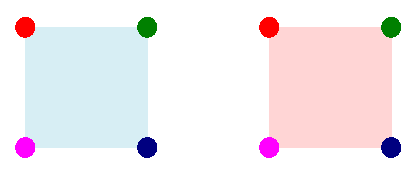
\includegraphics{figs/staggHypercubes.pdf}
  \caption{Example subdivision of one direction into disjoint hypercubes.
           Each hypercube is labeled by $h$, and the field $q(h)$
           associated to the hypercube is a linear combination of the
           $\chi$ fields on the corners, here represented by
           different colors. The effective lattice spacing between
           a $\chi$ of one corner of the blue hypercube and the corresponding
           $\chi$ in the same corner of the red hypercube is $a'=2a$.
           }
  \label{fig:staggHypercubes}
\end{figure}

We are now ready to carry out the substitution. The mass term follows
straightforwardly from the completeness relation. The kinetic term is
difficult, however, because the site offsets mix hypercubes. Therefore
it is crucially important to keep track of which hypercube $\chi$
belongs to. Keeping track of the hypercube will make manifest an $s$
dependence that makes applying the completeness relation not possible,
at least superficially. Gattringer and Lang~\cite{gattringer_quantum_2010}
suggest the following trick: we can shift the site that the first
hypercube starts on by one, which gives equivalent results as the
original hypercube labeling convention, and then average over these
two conventions. I was not able to figure this out. 
Rothe~\cite{rothe_lattice_2005} has another strategy, which I was also
not able to follow through. Nevertheless, one should find
\begin{equation}
S_F^{\rm stag}=a'^4\sum_h\Big(m\tr\left[\bar{q}q\right]
+\tr\left[\bar{q}\gamma_\mu\partial_\mu q\right]
-\frac{a'}{2}\tr\left[\bar{q}\gamma_5\Box_\mu q\gamma_\mu\gamma_5\right]\Big)
\end{equation}
where we have an implied summation over $\mu$, we have written
$q=q(h)$, introduced the effective spacing $a'\equiv2a$, and 
the discretized derivatives are
\begin{equation}
  \partial_\mu f(h)\equiv\frac{f(h+\hat{\mu})-f(h-\hat{\mu})}{2a'}
\end{equation}
and
\begin{equation}
  \Box_\mu f(h)\equiv\frac{f(h+\hat{\mu})-2f(h)+f(h-\hat{\mu})}{a'^2}.
\end{equation}

Our final step in the exploration of the staggered action will be to
identify the unphysical fermions. These {\it tastes} are hidden in
\index{taste}
the $q$. This should not be surprising because the $q_{ab}$ have 16
components, but Dirac spinors should have 4. This
tells us each $q$ corresponds to 4 spinors, and we will identify from
the $a$ and $b$ a taste index and Dirac index.
By comparing e.g. the $\tr[\bar{q}q]=\bar{q}_{ab}q_{ba}$ term with
what we expect from the physical, continuum theory, it makes sense
to identify the Dirac index with $b$. Thus our taste spinors are
\begin{equation}
  \psi^{t}(h)_\alpha\equiv q(h)_{\alpha t}~~~~\text{and}~~~~
  \bar{\psi}^{t}(h)_\alpha\equiv \bar{q}(h)_{t\alpha}.
\end{equation}
The staggered fermion action then becomes
\begin{equation}\label{eq:staggPhys}
S_F^{\rm stag}=a'^4\sum_h\left(
m\bar{\psi}^{t}\psi^{t}
+\bar{\psi}^{t}\gamma_\mu\partial_\mu\psi^{t}
-\frac{a'}{2}\bar{\psi}^{t}\gamma_5(\tau_5\tau_\mu)_{tt'}\Box_\mu\psi^{t'}
\right),
\end{equation}
where we have introduced new matrices
\begin{equation}
\tau_\mu\equiv\gamma_\mu^T.
\end{equation}

With the staggered action in the form of \equatref{eq:staggPhys} we can
begin to discuss some physics. The last term is called the
\index{taste!breaking}
{\it taste-breaking} term. It is similar to the Wilson term, in the
sense that it also represents a second derivative. However unlike
the Wilson term, it allows for interactions between fermions of
\index{taste!mixing}
different taste, i.e. it allows for {\it taste mixing}. If not for
the taste-breaking term, fermions of different taste would be mass-degenerate,
which one sees clearly from the first term. In the naive continuum limit,
this taste breaking terms vanishes like $a$.

The Wilson term broke axial symmetry completely, but in the taste-breaking
term, the remnant $\U_A(1)\times\U_A(1)$ remains. In particular this
term is invariant under transformations
\begin{equation}
\psi'=e^{i\omega}\psi, ~~~~~~
          \bar{\psi}'=\bar{\psi}e^{-i\omega}
\end{equation}
and
\begin{equation}
   \psi'=e^{i\omega\gamma_5\otimes\tau_5}\psi, ~~~~~~
          \bar{\psi}'=\bar{\psi}e^{i\omega\gamma_5\otimes\tau_5}.
\end{equation}
This latter symmetry follows from the fact that $\gamma_5$ commutes through
the taste-breaking term, while $\tau_5$ will pick up a minus sign.
One can identify this symmetry with a subgroup of the axial taste
symmetry group $\SU_A(N_t)$, where $N_t$ is the number of tastes.

At finite lattice spacing, taste mixing lifts the taste mass degeneracy.
One way to get some feeling for taste-breaking effects, then, is to look
at the mass spectrum of staggered fermions. It has been found that these
taste breaking effects can be reduced by improved gauge actions or smearing
\cite{durr_staggered_2004,follana_index_2004}, and in particular smearing
seems to drive masses to 4-fold degeneracy. An intuition for why smearing
might help is as follows: In the interacting theory, each $\chi$ is attached
to links according to its site, and since tastes are linear combinations
of these, it follows that different tastes touch different links. So
the more ``distance" in $\SU(N)$ space between the links, i.e. the more
the links fluctuate, the greater the taste-breaking effects will be.
Since smearing algorithms tend to drive links to more typical values
given their neighbors, they reduce these fluctuations, and hence
the taste-breaking.

We would also like to suppress the effects of unphysical tastes. Absent
taste-breaking, the Dirac operator corresponding to the staggered action
would be block diagonal in taste space, i.e. we would have for 
one physical flavor
\begin{equation}
D^{\rm stag}=\left(\begin{array}{cccc}
            D &   &  &  \\
              & D &  &  \\
              &   & D&  \\
              &   &  & D\\
            \end{array}\right).
\end{equation}
One commonly used strategy to remove the effects of taste-breaking is
\index{staggered!rooting}
therefore {\it rooting}. The idea is that $\det D^{\rm stag}$ is
the contribution to the probability distribution from four mass-degenerate
flavors. To isolate one of the flavors, it is sufficient to use
$\det D=(\det D^{\rm stag})^{1/4}$. For two degenerate light flavors
$m_l$ and one heavier flavor $m_s$, i.e. for $N_f=2+1$ fermions, 
one then samples with probability distribution
\begin{equation}\label{eq:HISQdist}
  \dd{\rm P}
    =\dd Ue^{-S_G}(\det D_l^{\rm stag})^{1/2}(\det D_s^{\rm stag})^{1/4}.
\end{equation}

In practice, taste-breaking is present at each lattice spacing, and
therefore it is not clear whether there is some leftover effect of rooting
in the continuum limit. In spite of this danger, people who employ staggered
actions often tend to use rooting anyway. One way to make this step more
justified is to reduce taste-breaking effects. Improved 
actions\footnote{We will discuss improved actions in more detail in 
\chref{ch:improve}.} such
as the HISQ action, to be discussed in the next section, have greatly
reduced taste-breaking and, reassuringly, results from HISQ actions
seem to agree with experiment.

%\section{Overlap fermions}

\section{Hadron interpolators}\label{sec:interpolators}

One of the goals of LQCD calculations is to learn something about hadrons. A
lattice operator that is supposed to represent some particular observable is
called an {\it interpolator}\index{interpolator}. Hence to learn something
about hadrons, we need to construct their corresponding interpolators. We follow
the presentation in Ref.~\cite{gattringer_quantum_2010}.

The guiding principles to constructing interpolators are:
\begin{enumerate}
  \item They are local, i.e. they should create/annihilate the particle of
        interest at a particular space-time point.
  \item They should be constructed from the quark fields that make the particle
        of interest.
  \item They need to have quantum numbers matching the particle of interest,
        e.g. they need to have the correct isospin, parity, electric charge,
        etc.
\end{enumerate} 
As an example, let us take the\index{interpolator!pion} pions. They are known to
have\footnote{These properties are determined experimentally. For
example the pion parity was found in the 1950s~\cite{chinowsky_reaction_1955}.} 
the quantum numbers $J=0$, $P=-1$, and $I=1$. There are three
pions, $\pi^{\pm}$ and $\pi^0$ with electric charges $\pm1$ and 0,
respectively; thus according to \tabref{tab:discreteSymm},
\secref{sec:isohyper}, and the above rules, we must have\footnote{The relative
minus sign in $\pi^0$ is to get $I_z=0$.}
\begin{equation}\begin{aligned}
  \pi^+(x) &= \bar{d}(x)\gamma_5u(x),\\
  \pi^-(x) &= \bar{u}(x)\gamma_5d(x),\\
  \pi^0(x) &= \frac{1}{\sqrt{2}}\left( \bar{u}(x)\gamma_5u(x)
                                      -\bar{d}(x)\gamma_5d(x)\right).
\end{aligned}\end{equation}
These interpolators correspond to the pion operators in our physical Hilbert
space; they annihilate a pion at $x$. Furthermore they are form an
isospin triplet.\index{triplet state} There is also a $u$, $d$ combination
with $I=0$, an isospin singlet state\index{singlet state}
\begin{equation}
\eta_{\rm non-phys.}(x)= \frac{1}{\sqrt{2}}\left( \bar{u}(x)\gamma_5u(x)
                                      +\bar{d}(x)\gamma_5d(x)\right),
\end{equation}
which can be interpreted as a kind of $\eta$\index{meson!$\eta$} 
meson.\footnote{The physical $\eta$ and $\eta'$ mesons are formed by 
$$
\eta= \frac{1}{\sqrt{6}}\left( \bar{u}u+\bar{d}d-2\bar{s}s\right)~~~~~
\eta'= \frac{1}{\sqrt{3}}\left( \bar{u}u+\bar{d}d+\bar{s}s\right).
$$
}

In general, meson interpolators have the
form
\begin{equation}\label{eq:mesonInterp}
 X=\bar{\psi}^f\Gamma\psi^g
\end{equation}
for some quarks $f$ and $g$. It turns out that to create meson $X$ one needs
\begin{equation}
 \bar{X}=\bar{\psi}^g\Gamma\psi^f.
\end{equation}

With the interpolators in hand, we can construct general meson correlators.
A correlation function\index{correlator} 
that creates a meson $X$ at $y$ and annihilates it at $x$ is
\begin{equation}
  G(x,y)\equiv\bra{0}X(x)\bar{X}(y)\ket{0}=\ev{X(x)\bar{X}(y)}.
\end{equation} 
We now recast this equation in a form more practical for lattice calculations.
In particular we focus on expectation values $\ev{...}_F$. From
\equatref{eq:deffermev} we see that these expectation values can be factorized
according to quark flavor, which will be useful to us. As we will see,
isotriplet and isosinglet operators will have slightly different forms.

To start, we consider simple isotriplet operators of the form
$X=\bar{d}\Gamma u$. Expressing Lorentz and color indices explicitly we obtain 
\begin{equation}\begin{aligned}\label{eq:contraction}
\ev{X(x)\bar{X}(y)}_F&=\ev{\bar{d}(x)\Gamma u(x)\bar{u}(y)\Gamma d(y)}_F\\
&=
\Gamma_{\alpha\beta}\Gamma_{\bar{\alpha}\bar{\beta}}
\ev{\bar{d}(x)_{\alpha c}u(x)_{\beta c}\bar{u}(y)_{\bar\alpha\bar
c}d(y)_{\bar\beta \bar c}}_F\\
&=
-\Gamma_{\alpha\beta}\Gamma_{\bar{\alpha}\bar{\beta}}
\ev{u(x)_{\beta c}\bar{u}(y)_{\bar\alpha\bar c}}_u
\ev{d(y)_{\bar\beta \bar c}\bar{d}(x)_{\alpha c}}_d\\
&=
-\Gamma_{\alpha\beta}\Gamma_{\bar{\alpha}\bar{\beta}}
D^{-1}_u(x,y)_{\beta\bar\alpha c\bar c}
D^{-1}_d(y,x)_{\bar\beta\alpha \bar cc}\\
&=-\tr\left[\Gamma D_u^{-1}(x,y)\Gamma D_d^{-1}(y,x)\right],
\end{aligned}\end{equation}
where we used Wick's theorem to arrive at fourth line.
Through Wick's theorem, the original correlation function can be expressed in
terms a trace of product of gamma matrices $D^{-1}$ operators that originally
appeared in the fermionic part of the action. 

\begin{figure}
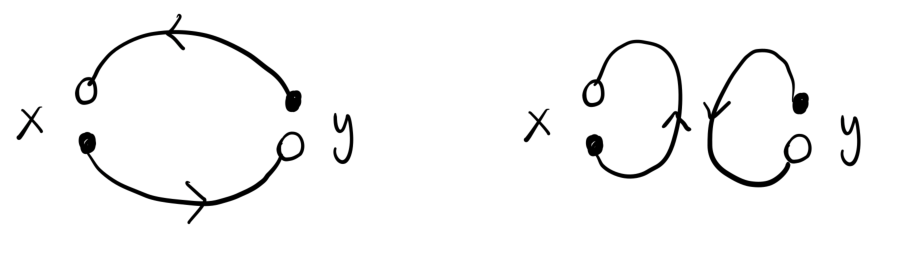
\includegraphics[width=\textwidth]{figs/connected_disconnected.pdf}
\caption{Examples of connected (left) and disconnected (right) diagrams
between spacetime points $x$ and $y$. The arrows indicate the direction of
propagation. Any vertical pair of open and closed circles can be interpreted as
a meson.}
\label{fig:contraction}
\end{figure}

The above computation is an example of a fermion {\it contraction}\index{contraction}.
Equation \eqref{eq:contraction} can be interpreted as follows: The propagator
$D^{-1}_u$ propagates a $u$ quark from $y$ to $x$; simultaneously, the
$D^{-1}_d$ propagates a $d$ quark from $x$ to $y$. The corresponding Feynman
diagram is referred to as a {\it connected}\index{connected diagram} 
diagram. This is shown
schematically in \figref{fig:contraction} (left).\footnote{By doing a hopping
parameter expansion, one can show that $D^{-1}$ can be expressed as a weighted
sum over all possible, non-backtracking paths from $y$ to $x$. So the directed lines 
shown in the \figref{fig:contraction} can be thought of as shorthand
for such sums.}

Using the same kinds of manipulations as in the contraction
\eqref{eq:contraction}, one can show that correlators of 
isosinglet operators of the form
$X=\left(\bar{u}\Gamma u+\bar{d}\Gamma d\right)/\sqrt{2}$ become
\begin{equation}\begin{aligned}\label{eq:disconnectedContribution}
2\ev{X(x)\bar{X}(y)}_F&=
-\tr\left[\Gamma D_u^{-1}(x,y)\Gamma D_u^{-1}(y,x)\right]\\
&~~~~+\tr\left[\Gamma D_u^{-1}(x,x)\right]\tr\left[\Gamma D_u^{-1}(y,y)\right]\\
&~~~~+\tr\left[\Gamma D_u^{-1}(x,x)\right]\tr\left[\Gamma D_d^{-1}(y,y)\right]
+(u\leftrightarrow d).
\end{aligned}\end{equation}
Here we see the appearance of {\it disconnected}\index{disconnected diagram}
diagrams, like $\tr\Gamma D^{_1}(x,x)$, which can be visualized as in
\figref{fig:contraction} (right). These diagrams propagate a quark from a point
$x$ back to $x$. Correlators of the form
$X=\left(\bar{u}\Gamma u-\bar{d}\Gamma d\right)/\sqrt{2}$, like the $I_z=0$
component of the isotriplet, are exactly the same as
\equatref{eq:disconnectedContribution}, except that there appears a relative
minus sign between $u$ and $d$ terms. Computations that set $m_u=m_d$, i.e.
{\it isospin symmetric}\index{isospin!symmetric calculation} calculations, have
the benefit that the disconnected pieces cancel out. This turns out to be
especially convenient, as disconnected diagrams are more expensive to
compute than connected ones.

We note that states of definite spatial momentum $\vec{p}$ can be obtained by
Fourier transforming out the spatial sites, similar to \equatref{eq:fourierLat}.
In this way, the time component $t$ is left free, and the resulting
transform $\tilde{X}\left(\vec{p},t\right)$, being a sum over all sites on the
time-slice $t$, is interpreted as living on the time-slice. 

We close by giving a final formula to compute hadron correlators on the lattice,
exemplifying the case of a connected meson interpolator. Combining
Eqs.~\eqref{eq:evfact}, \eqref{eq:evferm}, \eqref{eq:contraction}, and
the Matthews-Salam formula, we arrive at
\begin{equation}\label{eq:mesonCorrFormula}
\ev{X(x)\bar{X}(y)}=-\frac{1}{Z}
\int\DD U e^{-S_G}\det D_u\det D_d \tr\left[\Gamma D_u^{-1}(x,y)\Gamma
D_d^{-1}(y,x)\right].
\end{equation}

\section{Pseudofermions}\label{sec:pseudofermions}

As discussed in \secref{sec:grassmann}, the Matthews-Salam formula
lets us integrate out the fermion fields, and we are left with
the determinant of a very large matrix, the Dirac matrix, in
our integration measure. Computing this determinant directly
is not computationally feasible. Let us follow a nice presentation
from Ref.~\cite{degrand_lattice_2006} to learn how to approach
simulating dynamical fermions in spite of this difficulty.

The partition function for a single fermion species is
\begin{equation}\begin{aligned}
  Z&=\int\DD U\DD\bar\psi\DD\psi e^{-S_G-\bar\psi D\psi}
   &=\int\DD U \det D\,e^{-S_G}.
\end{aligned}\end{equation}
As we can see in \eqref{eq:diracPositionBasis}, we think of $D$ as a matrix in
the basis of space-time sites, i.e. there is an element for each pair of
space-time points. Even though it is a sparse matrix, its dimensionality is
still impossibly huge, and hence computing determinants in a straightforward
manner is computationally not feasible\footnote{As discussed with
staggered fermions, we will want to take
square roots and fourth roots of the Dirac operator. These rooted matrices
have even more nonzero entries, exacerbating the problem significantly.
It should be that the further one gets from the diagonal, the smaller
the entries become, and in the continuum limit, $D$ 
should become local\index{local}. It should be noted that
the time complexity of
computing the determinant of an $N\times N$ matrix
is usually $\order{N^3}$. This is of course algorithm-dependent,
but the lowest I am aware of is still
slower than $\order{N^2}$, which for us would correspond to
the lattice volume squared.}. 

Instead of evaluating the determinant, we approximate it
by introducing 
{\it pseudofermions}~\cite{fucito_proposal_1981,weingarten_physics_1981}.
A pseudofermion $\Phi\equiv\Phi_R+i\Phi_I$ is a color-triplet, complex, 
scalar field. We leverage the formal identity
\begin{equation}\label{eq:pseudofermionIdentity}
\det M \sim \int\DD{\Phi_R}\DD{\Phi_I}\exp\left(-\Phi^\dagger M^{-1}\Phi\right),
\end{equation}
where the squiggle indicates there may be some irrelevant factors 
missing\footnote{Remember that the only important thing when it comes to
predicting observables is that expectation values remain unchanged.
Constant factors always drop out in the ratio. In Gattringer and Lang I
see some factors $\pi^N$, which I do not always see in the literature.}.
Now, it is always crucial that our exponentials can be interpreted
as probabilities; therefore an important question to ask is whether
that exponential is real and bounded.

One way to explore the argument of the above exponential is to decompose
the scalar fields $\Phi$ in terms of eigenvectors of $M$. Assuming $M$
is an $N\times N$ matrix with only nonzero eigenvalues $\lambda_i$, 
we can write
\begin{equation}
\Phi^\dagger M^{-1}\Phi=\sum_{i=1}^N
\left(\Phi^\dagger\psi\right)_i\frac{1}{\lambda_i}\left(\psi^\dagger\Phi\right)_i.
\end{equation}
The projections of $\Phi$ onto the eigenstates of $M$ are complex
conjugates, so if the eigenvalues were positive, we would be guaranteed that
$\Phi^\dagger M^{-1}\Phi$ is positive. The trick then is to look
out for an operator $M$ with positive eigenvalues.

In \secref{sec:signProblem} we will see that most Dirac operators $D$ used in
lattice field theory are $\gamma_5$-hermitian\index{hermitian},
which means they obey
\begin{equation}
D^\dagger=\gamma_5 D \gamma_5.
\end{equation}
In that Section, we will show this guarantees
\begin{equation}
\det D = \det D^\dagger,
\end{equation}
and hence if we choose $M=D^\dagger D$, we will have
by \equatref{eq:pseudofermionIdentity}
\begin{equation}\label{eq:twoPseudofermionFlavors}
\left(\det D\right)^2 
=\det D^\dagger D 
\sim \int\DD{\Phi_R}\DD{\Phi_I}
\exp\left(-\Phi^\dagger \left(D^\dagger D\right)^{-1}\Phi\right),
\end{equation}
i.e. we will be able to rewrite the fermion determinants corresponding
to a system with two identical flavors of quark in a way that guarantees
we can use a Markov chain.

An important practical point to consider is how to generate $\Phi$ according to
the distribution \equatref{eq:twoPseudofermionFlavors}. Let $R$ be a random
vector such that
\begin{equation}
\Phi=D^\dagger R.
\end{equation}
Then if we draw $R$ from a Gaussian, i.e. if we draw
according to $\exp\left(-R^\dagger R\right)$, we are guaranteed that
$\Phi$ will be distributed as desired.
\bibliographystyle{unsrtnat}
\bibliography{bibliography}
